\subsubsection{Assíncronos}

Contadores assíncronos, também conhecidos como contadores \textit{ripple}, são aqueles em que os flip-flops não compartilham um sinal de clock global. Em vez disso, a saída de cada flip-flop é utilizada como sinal de clock para o próximo estágio.

Essa estrutura faz com que as transições de estado ocorram de forma sequencial, propagando-se ao longo do circuito. Esse fenômeno, denominado \textit{ripple}, introduz atrasos acumulados entre os bits, uma vez que cada flip-flop depende da estabilização do anterior.

\begin{figure}[H]
   	\centering
   	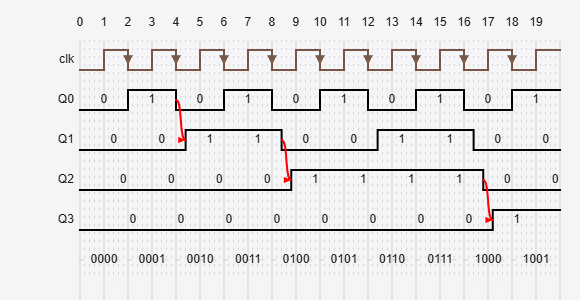
\includegraphics[width=0.6\linewidth]{images/assincrono-time-diagram.png}
  	 \caption{Diagrama de tempo de um contador assíncrono}
   	\label{fig:assincrono-time-diagram}
\end{figure}

Como consequência, durante as transições, o sistema pode assumir estados intermediários inválidos por curtos intervalos de tempo, o que compromete a previsibilidade temporal do circuito.

Apesar disso, contadores assíncronos apresentam baixa complexidade estrutural, uma vez que não requerem lógica combinacional adicional para controle de transição. Por essa razão, são frequentemente utilizados em aplicações simples, onde custo e facilidade de implementação são mais relevantes do que precisão temporal.

Tipicamente, esses contadores são implementados com flip-flops JK conectados em cascata, conforme ilustrado a seguir:

\begin{figure}[H]
   	\centering
   	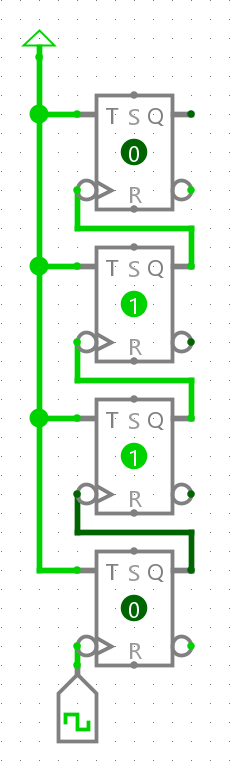
\includegraphics[width=0.14\linewidth]{images/assincrono-circuit.png}
  	 \caption{Circuito de um contador assíncrono}
   	\label{fig:assincrono-circuit}
\end{figure}